% 图 3.6 Mn3+（3d4）的 Jahn--Teller 效应：
% 上：能级沿畸变展开（按物理：沿 z 伸长使 d_z2 下降并被占据，d_x2-y2 升高为空）
% 下：正八面体 -> 沿 z 伸长的畸变八面体
\documentclass[tikz,border=5pt]{standalone}
\usetikzlibrary{arrows.meta}
\usepackage{amsmath}
\usepackage{bm}
\usepackage{fontspec}
\setmainfont{Times New Roman}
\begin{document}
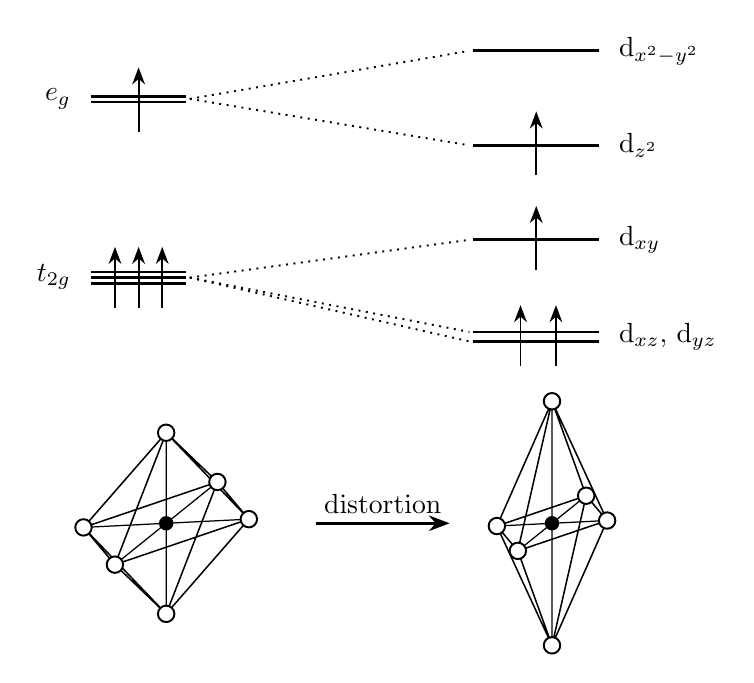
\begin{tikzpicture}[line width=0.8pt,>=Stealth,
  lvl/.style={line width=1.0},
  fan/.style={line width=0.7,dotted}]
% ================ 上半：能级图 ================
% 左：未畸变 e_g（二重，1 个电子）与 t_2g（三重，3 个电子）
\node[anchor=east] at (0.42,6.94) {$e_g$};
\draw[lvl] (0.55,6.90) -- (1.75,6.90);
\draw[lvl] (0.55,6.97) -- (1.75,6.97);
\draw[->,line width=0.7] (1.15,6.52) -- (1.15,7.34);
\node[anchor=east] at (0.42,4.68) {$t_{2g}$};
\draw[lvl] (0.55,4.60) -- (1.75,4.60);
\draw[lvl] (0.55,4.67) -- (1.75,4.67);
\draw[lvl] (0.55,4.74) -- (1.75,4.74);
\foreach \x in {0.85,1.15,1.45}{\draw[->,line width=0.7] (\x,4.28) -- (\x,5.06);}
% 点线扇形展开
\draw[fan] (1.80,6.94) -- (5.35,7.55);
\draw[fan] (1.80,6.94) -- (5.35,6.35);
\draw[fan] (1.80,4.67) -- (5.35,5.15);
\draw[fan] (1.80,4.67) -- (5.35,3.98);
\draw[fan] (1.80,4.67) -- (5.35,3.86);
% 右：畸变后能级（自上而下：d_x2-y2 空、d_z2(1e)、d_xy(1e)、d_xz=d_yz(2e)）
\draw[lvl] (5.40,7.55) -- (7.00,7.55);
\node[anchor=west] at (7.12,7.55) {$\mathrm{d}_{x^2-y^2}$};
\draw[lvl] (5.40,6.35) -- (7.00,6.35);
\draw[->,line width=0.7] (6.20,5.97) -- (6.20,6.78);
\node[anchor=west] at (7.12,6.35) {$\mathrm{d}_{z^2}$};
\draw[lvl] (5.40,5.15) -- (7.00,5.15);
\draw[->,line width=0.7] (6.20,4.77) -- (6.20,5.58);
\node[anchor=west] at (7.12,5.15) {$\mathrm{d}_{xy}$};
\draw[lvl] (5.40,3.98) -- (7.00,3.98);
\draw[lvl] (5.40,3.86) -- (7.00,3.86);
\draw[->,line width=0.7] (6.00,3.55) -- (6.00,4.32);
\draw[->,line width=0.7] (6.45,3.55) -- (6.45,4.32);
\node[anchor=west] at (7.12,3.92) {$\mathrm{d}_{xz}$, $\mathrm{d}_{yz}$};
% ================ 下半：八面体畸变 ================
% 左：正八面体
\begin{scope}[shift={(1.50,1.55)},x={(-0.62cm,-0.50cm)},y={(1cm,0.05cm)},z={(0,1cm)}]
\draw[line width=0.55]
  (0,0,1.15) -- (0,1.05,0)   (0,0,1.15) -- (1.05,0,0)
  (0,0,1.15) -- (0,-1.05,0)  (0,0,1.15) -- (-1.05,0,0)
  (0,0,-1.15) -- (0,1.05,0)  (0,0,-1.15) -- (1.05,0,0)
  (0,0,-1.15) -- (0,-1.05,0) (0,0,-1.15) -- (-1.05,0,0)
  (0,1.05,0) -- (1.05,0,0)   (1.05,0,0) -- (0,-1.05,0)
  (0,-1.05,0) -- (-1.05,0,0) (-1.05,0,0) -- (0,1.05,0);
\draw[line width=0.45]
  (0,0,0) -- (0,0,1.15)  (0,0,0) -- (0,0,-1.15)
  (0,0,0) -- (0,1.05,0)  (0,0,0) -- (0,-1.05,0)
  (0,0,0) -- (1.05,0,0)  (0,0,0) -- (-1.05,0,0);
\node[circle,draw,fill=white,inner sep=2.1pt,line width=0.7] at (0,0,1.15) {};
\node[circle,draw,fill=white,inner sep=2.1pt,line width=0.7] at (0,0,-1.15) {};
\node[circle,draw,fill=white,inner sep=2.1pt,line width=0.7] at (0,1.05,0) {};
\node[circle,draw,fill=white,inner sep=2.1pt,line width=0.7] at (0,-1.05,0) {};
\node[circle,draw,fill=white,inner sep=2.1pt,line width=0.7] at (1.05,0,0) {};
\node[circle,draw,fill=white,inner sep=2.1pt,line width=0.7] at (-1.05,0,0) {};
\fill (0,0,0) circle (2.6pt);
\end{scope}
% distortion 箭头
\draw[->,line width=1.0] (3.40,1.55) -- (5.10,1.55);
\node at (4.25,1.80) {distortion};
% 右：沿 z 伸长的八面体
\begin{scope}[shift={(6.40,1.55)},x={(-0.62cm,-0.50cm)},y={(1cm,0.05cm)},z={(0,1cm)}]
\draw[line width=0.55]
  (0,0,1.55) -- (0,0.70,0)   (0,0,1.55) -- (0.70,0,0)
  (0,0,1.55) -- (0,-0.70,0)  (0,0,1.55) -- (-0.70,0,0)
  (0,0,-1.55) -- (0,0.70,0)  (0,0,-1.55) -- (0.70,0,0)
  (0,0,-1.55) -- (0,-0.70,0) (0,0,-1.55) -- (-0.70,0,0)
  (0,0.70,0) -- (0.70,0,0)   (0.70,0,0) -- (0,-0.70,0)
  (0,-0.70,0) -- (-0.70,0,0) (-0.70,0,0) -- (0,0.70,0);
\draw[line width=0.45]
  (0,0,0) -- (0,0,1.55)  (0,0,0) -- (0,0,-1.55)
  (0,0,0) -- (0,0.70,0)  (0,0,0) -- (0,-0.70,0)
  (0,0,0) -- (0.70,0,0)  (0,0,0) -- (-0.70,0,0);
\node[circle,draw,fill=white,inner sep=2.1pt,line width=0.7] at (0,0,1.55) {};
\node[circle,draw,fill=white,inner sep=2.1pt,line width=0.7] at (0,0,-1.55) {};
\node[circle,draw,fill=white,inner sep=2.1pt,line width=0.7] at (0,0.70,0) {};
\node[circle,draw,fill=white,inner sep=2.1pt,line width=0.7] at (0,-0.70,0) {};
\node[circle,draw,fill=white,inner sep=2.1pt,line width=0.7] at (0.70,0,0) {};
\node[circle,draw,fill=white,inner sep=2.1pt,line width=0.7] at (-0.70,0,0) {};
\fill (0,0,0) circle (2.6pt);
\end{scope}
\end{tikzpicture}
\end{document}
